\documentclass[12pt, letterpaper]{report}
\usepackage[utf8]{inputenc}
\usepackage[T1]{fontenc}
\usepackage[english,polish]{babel}
\usepackage{fancyhdr}
\usepackage{hyperref}

\usepackage{graphicx}
\graphicspath{ {images/} }

\usepackage[margin=1.5cm]{geometry}

\title{
    Raport z postępów pracy \\
    \large Modelowanie elastycznych i nieelastycznych
    zderzeń obiektów\\
    metodą dynamiki molekularnej na potrzeby animacji
    komputerowych
}
\author{
    Kamil Pasterczyk \\
    \small Promotor: dr hab. inż. Tomasz Chwiej
}

\begin{document}

\maketitle
\tableofcontents

\chapter{Wstęp}
    \section{Opis}
    First document. This is a simple example, with no
    extra parameters or packages included. Hello world, nice to meet you

\chapter{Rozwinięcie}
    \section{Opis rozwinięcia}

    \begin{figure}[h]
        \centering
        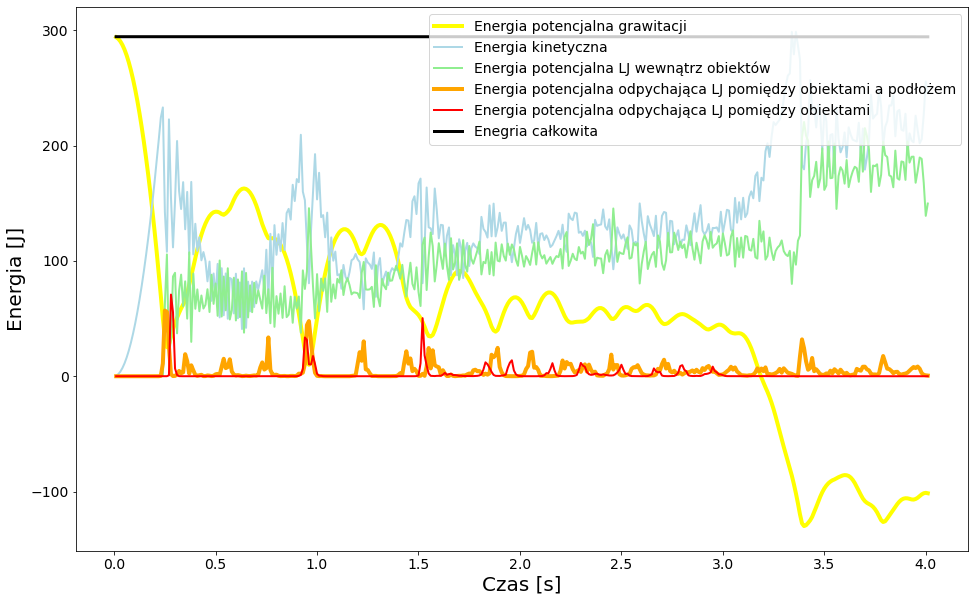
\includegraphics[width=16cm]{energy_test_0to4s}
        \caption{Zmiana enegii w czasie dla układu złożonego z dwóch obiektów i podłoża}
    \end{figure}

\chapter{Zakończenie}
    \section{Dodatek}

    \subsection{Filmik prezentujące działanie aplikacji}

    \subsubsection{Przekazanie energii między dwoma sztywnimi obiektami}

    Mniejszy obiekt $3 \times 3$ po odbiciu od większego obiektu $8 \times  8$ znajdującego się pod nim wznosi się na
    wysokość o wiele większą, niż ta z której rozpoczął spadek swobodny.
    Występuje tutaj przekazanie części energii z obiektu większego do mniejszego - sama zasada energii jest zachowana.

    \paragraph{
        \url{https://youtu.be/nolLh6CSa-8}
    }

    \subsubsection{Przekazanie energii między dwoma miękkimi obiektami}
    W tym przypadku obiekty są mniej sztywne,
    obiekt $3 \times 3$ po odbiciu od obiektu $8 \times  8$ wznosi się na wyraźnie mniejszą wysokość niż w przypadku bardziej sztywnych obiektów
    (jednak wciąż wyżej niż punkt z którego zaczął spadać). Można to wytłumaczyć tym,
    że znaczna część energii która w poprzednim przypadku była częścią ruchu postępowego,
    teraz stała się energią wewnętrzną obiektów (wibracje obiektów pochłaniają część energii).

    \paragraph{
        \url{https://youtu.be/q2uYx8uLl3w}
    }

    \subsubsection{Proste zderzenie dwóch obiektów}
    \paragraph{
        \url{https://www.youtube.com/watch?v=4cGcL_5yUt4}
    }

    \subsection{Inne}
    Repozytorium z kodem projektu
    \paragraph{
        \url{https://github.com/theYiome/elastic-objects-rs}
}

\end{document}